
\subsection{Particle Time of Flight and Energy Determination}
\label{ToF_reconstruction}
The ToF of detected particles is used to distinguish between neutrons and photons as well as determine neutron energy.
A particle's reconstructed position is used to determine direction of motion, which is then used to calculate the opening angle between pairs of detected particles.
Position and ToF are each determined using the timing of coincident signals from both PMTs of a given detector.

The sum of the times required for scintillation light to travel from the point of scintillation to both PMTs is equal to the time required for the light to travel the full length of the scintillator, which is a constant for light that travels parallel to the length of the scintillator.
This is supported by data, shown in Fig.~\ref{fig:ConstPMTAvg}, which were produced from a series of tests in which a collimated $^{60}$Co source was placed at seven different locations along a scintillator.
One of the two coincident photons emitted by $^{60}$Co reaches the scintillator and the other is detected by an auxiliary detector serving as the trigger. 
The photons incident on the scintillator have a spot size of less than 1~cm due to source collimation.
These events all have equal transit time, regardless of the $^{60}$Co source's position. %because the coincident photons are emitted simultaneously and the distance they must travel is unchanged. 

In Figure~\ref{fig:ConstPMTAvg}(a), it can be seen that the time required for the scintillation light to propagate along the scintillator has a large effect on the timing of each PMT alone, however, the average of the times of both PMTs is a constant, unaffected by the location at which the particle undergoes scintillation.
For this reason, taking the average of signals from two PMTs is advantageous because it removes the roughly 5~ns timing error that would otherwise exist due to the time required for scintillation light to propagate along the scintillator.
The requirement that there be coincident events in both of a detector's PMTs also aids in reducing noise.

\begin{figure}[]
\centering
\subfloat[]{\hspace{-0.5cm}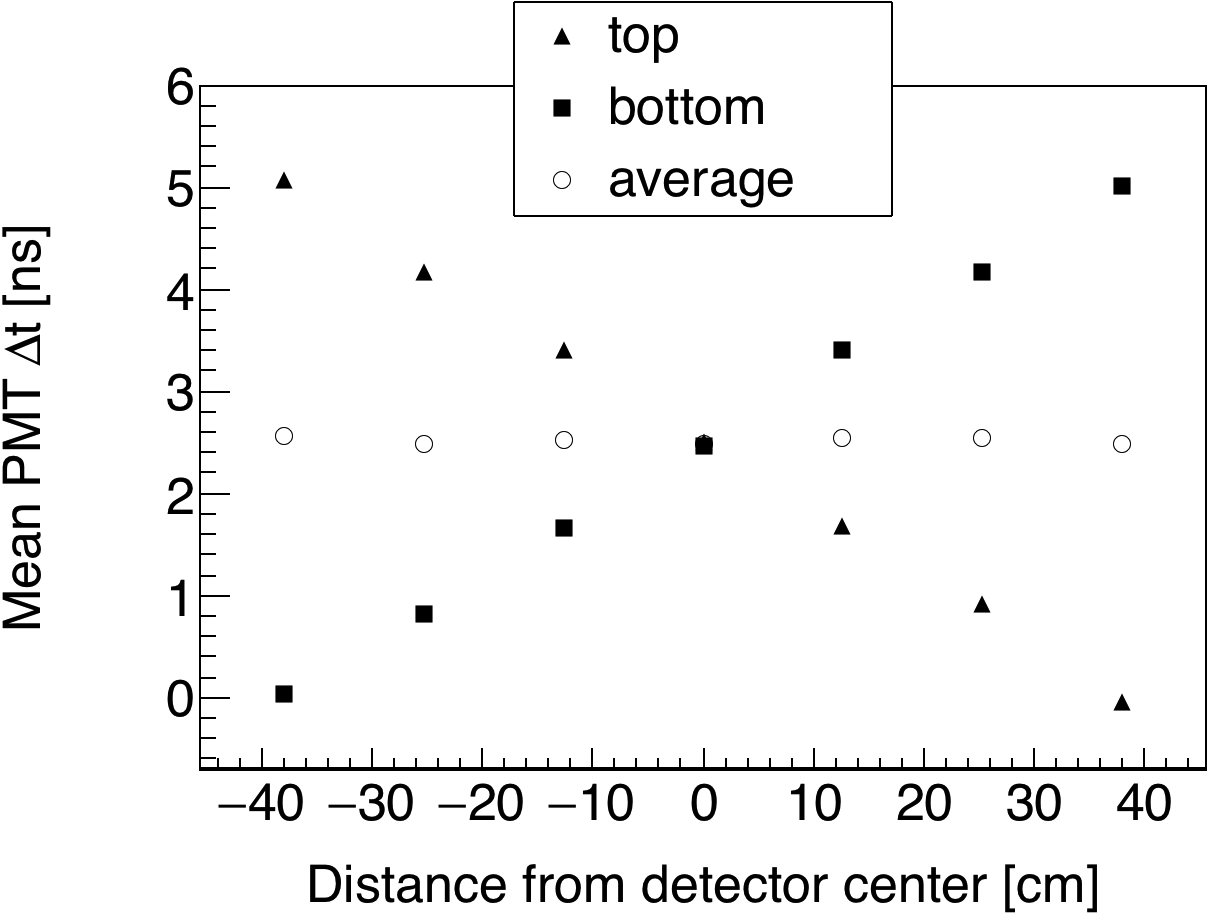
\includegraphics[width=\figsmall\textwidth]{ConstPMTAvg.png}}

\subfloat[]{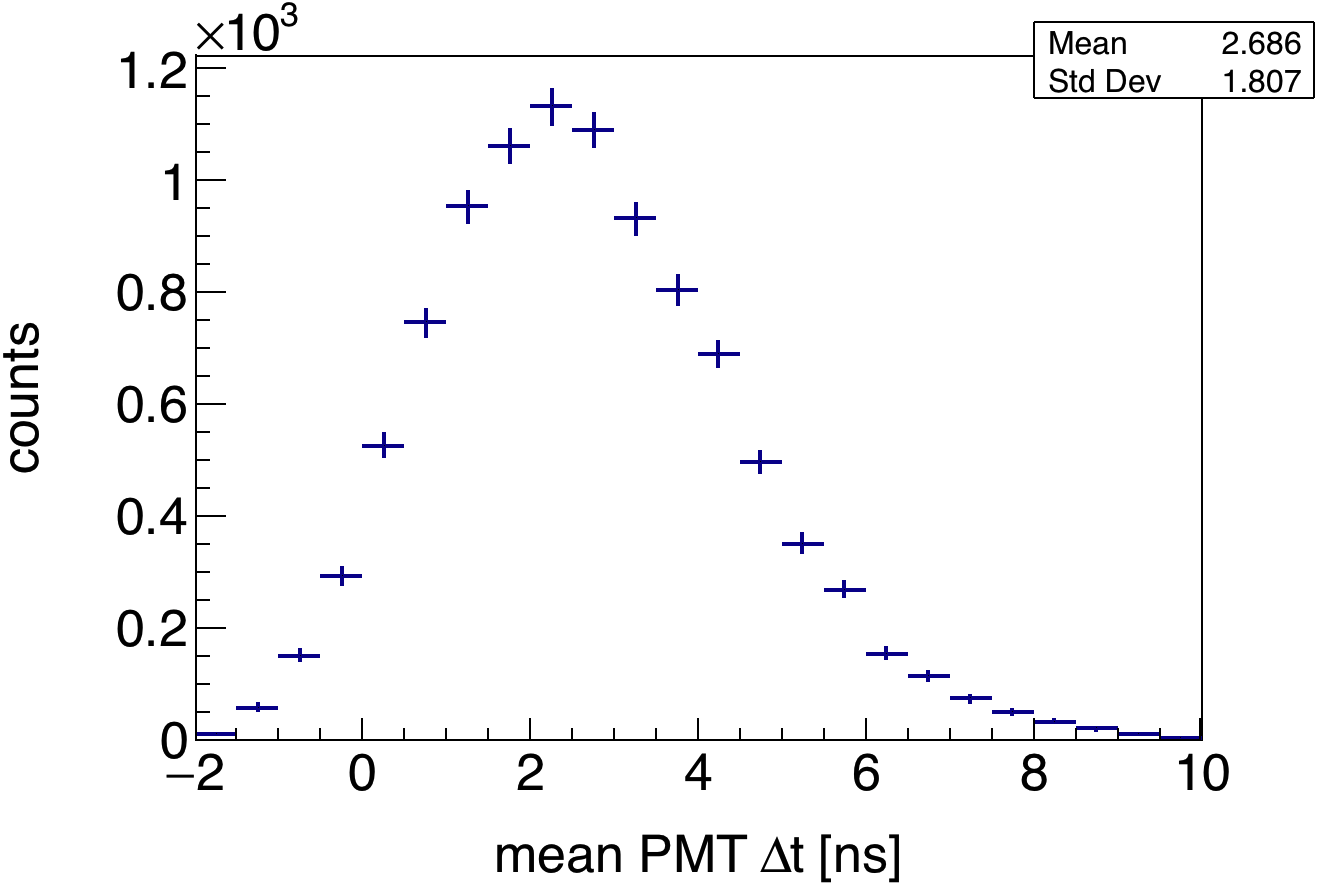
\includegraphics[width=\figsmall\textwidth]{ConstPMTAvgProject.png}}
\caption{A collimated $^{60}$Co source is used to produce photon events with constant ToF at seven locations along the detector.
$^{60}$Co produces coincident photons, and one is detected by the scintillator and the other by a separate trigger detector.
 $\Delta t$ is the timing of a PMT signal relative to a signal from the trigger detector. 
 In (a), it can be seen that the average between signals from both PMTs does not depend on position.
By using the PMT average, there is a reduction in error due to the time required for scintillation light to travel along the scintillator.
The uncertainty in ToF measurements is equal to the standard deviation seen in (b), or about $\pm$2~ns, because all photons from the $^{60}$Co source have the same ToF.}
\label{fig:ConstPMTAvg}
\end{figure}

During photofission measurements, ToF is calculated by the following expression:
\begin{equation}
\label{eq:ToF}
\text{ToF} = t^{PMTs}_{\text{mean}} - t_{\text{beam}} + C \, ,
\end{equation}
where $t^{PMTs}_{\text{mean}}$ is the mean of the times of signals from both PMTs of a scintillator, $t_{\text{beam}}$ is the time of a signal provided by the accelerator at the beginning of each pulse, and $C$ is a constant timing offset.
Any process that produces a timing delay that does not change from pulse to pulse contributes to $C$.
For example, the time required for photons to travel from the bremsstrahlung radiator to the target, the propagation of signals through the cables connecting the PMTs, delays in the electronics, {\em{etc}}.

\begin{figure}[]
\centering
    \subfloat[]{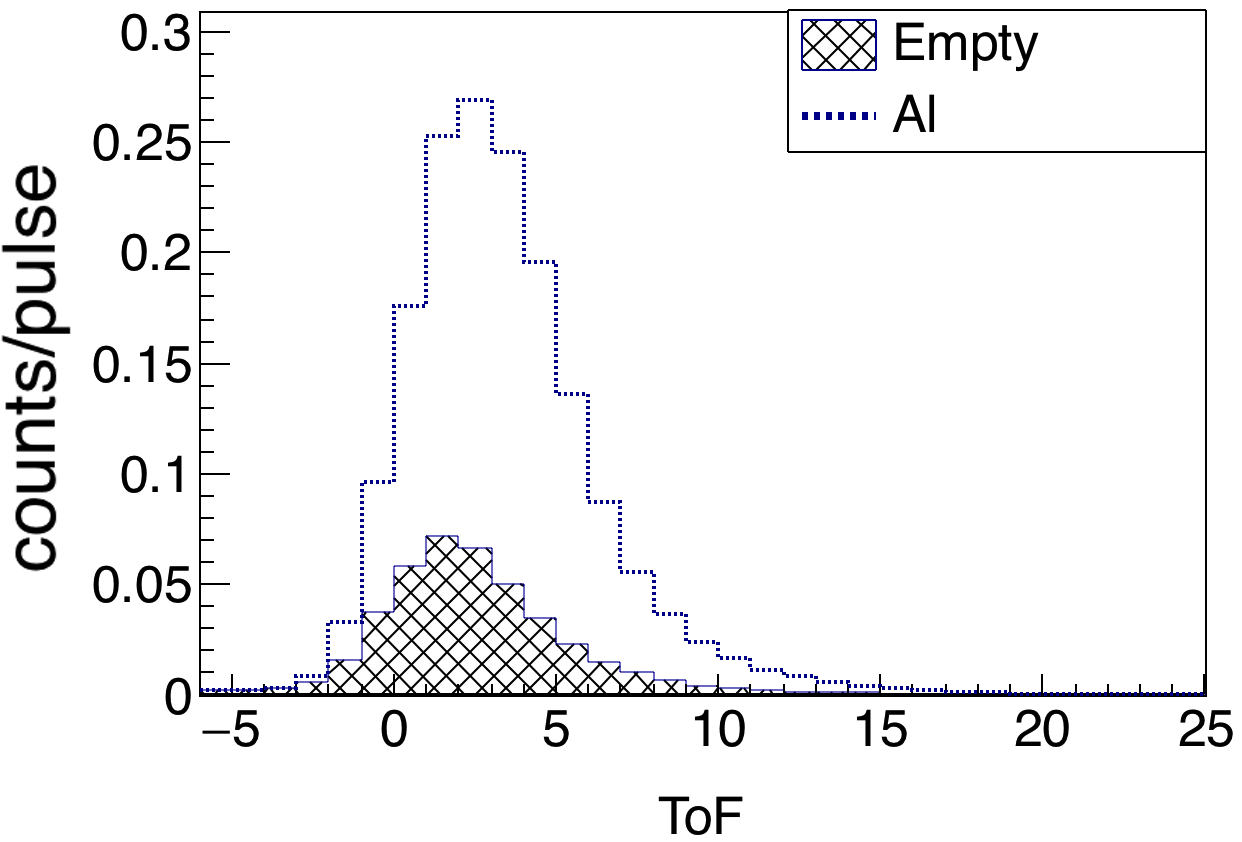
\includegraphics[width=\figsmall\textwidth]{MTvsAl.png}} \figToFNewline
    \subfloat[]{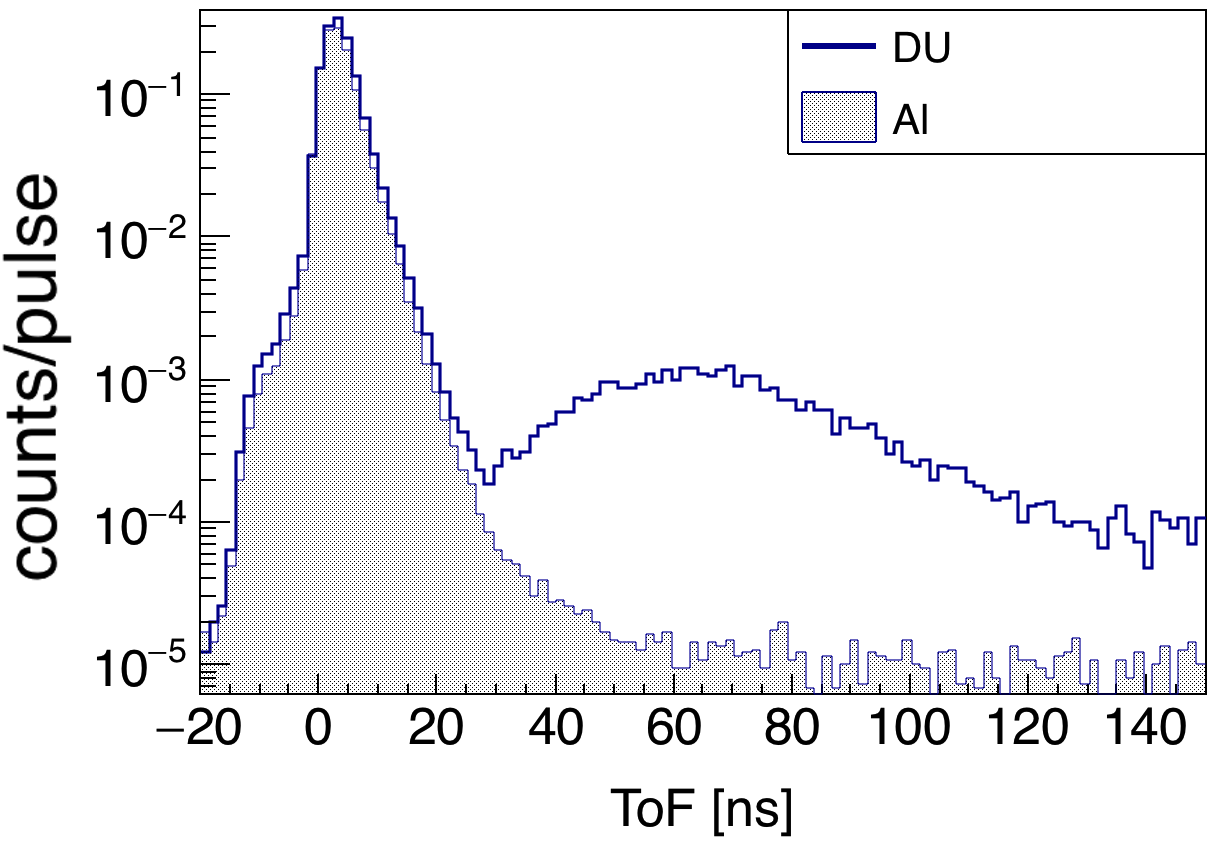
\includegraphics[width=\figsmall\textwidth]{DUvsAl.png}}
    \caption{(a) Comparison between the ToF spectrum of a non-neutron producing target made from Al, to the ToF spectrum produced when no target is used.
    The large increase in events around 4~ns is due to photons that scatter from the Al target.
    When no target is in place, sources of the peak include the collimator leading into the experimental cell and the beam dump.
    The photon peak seen here is used to find the timing offsets that make it so $t=0$ corresponds to the moment of fission.
    (b) Comparison between the Al and DU targets show a pronounced increase in events for DU between 35 and 130~ns due to the introduction of neutrons.}
    \label{fig:ToF}
\end{figure}

The value of $C$, which may be different for each detector, is determined by comparing the timing spectra of the gamma flash produced by a non-neutron producing aluminum target, to that produced when no target is used (see Fig.~\ref{fig:ToF}).
The difference between these two spectra reveals a prominent peak in the ToF spectrum due to photons that scatter from the aluminum target.
These photons must travel 125~cm to reach the center of any detector and 130~cm to reach the top, for which it takes light 4.2~ns and 4.3~ns to travel, respectively.
The value of $C$ used for each detector is equal to the value that places the time corresponding to the peak of the target-induced gamma flash at 4~ns.

%For 10 MeV neutrons, relativistic and non-relativistic energy calculations differ by about 1\%.
The kinetic energy of a detected neutron is determined straightforwardly from its velocity, which is determined from its ToF under the assumption that the neutron traveled directly from the target to the detectors unimpeded.
According to a series of MCNP simulations examining the scattering of fission neutrons within detector shielding and the fission target, neutrons predominantly travel to the detectors unimpeded.
These simulations are discussed in sections~\ref{subsection:targets} and \ref{subsection:detectors}.

Figure~\ref{fig:ErgUncertainty} shows the measurement uncertainty in neutron energy due to error in the ToF determination.
\begin{figure}[]
%    \subfloat[]{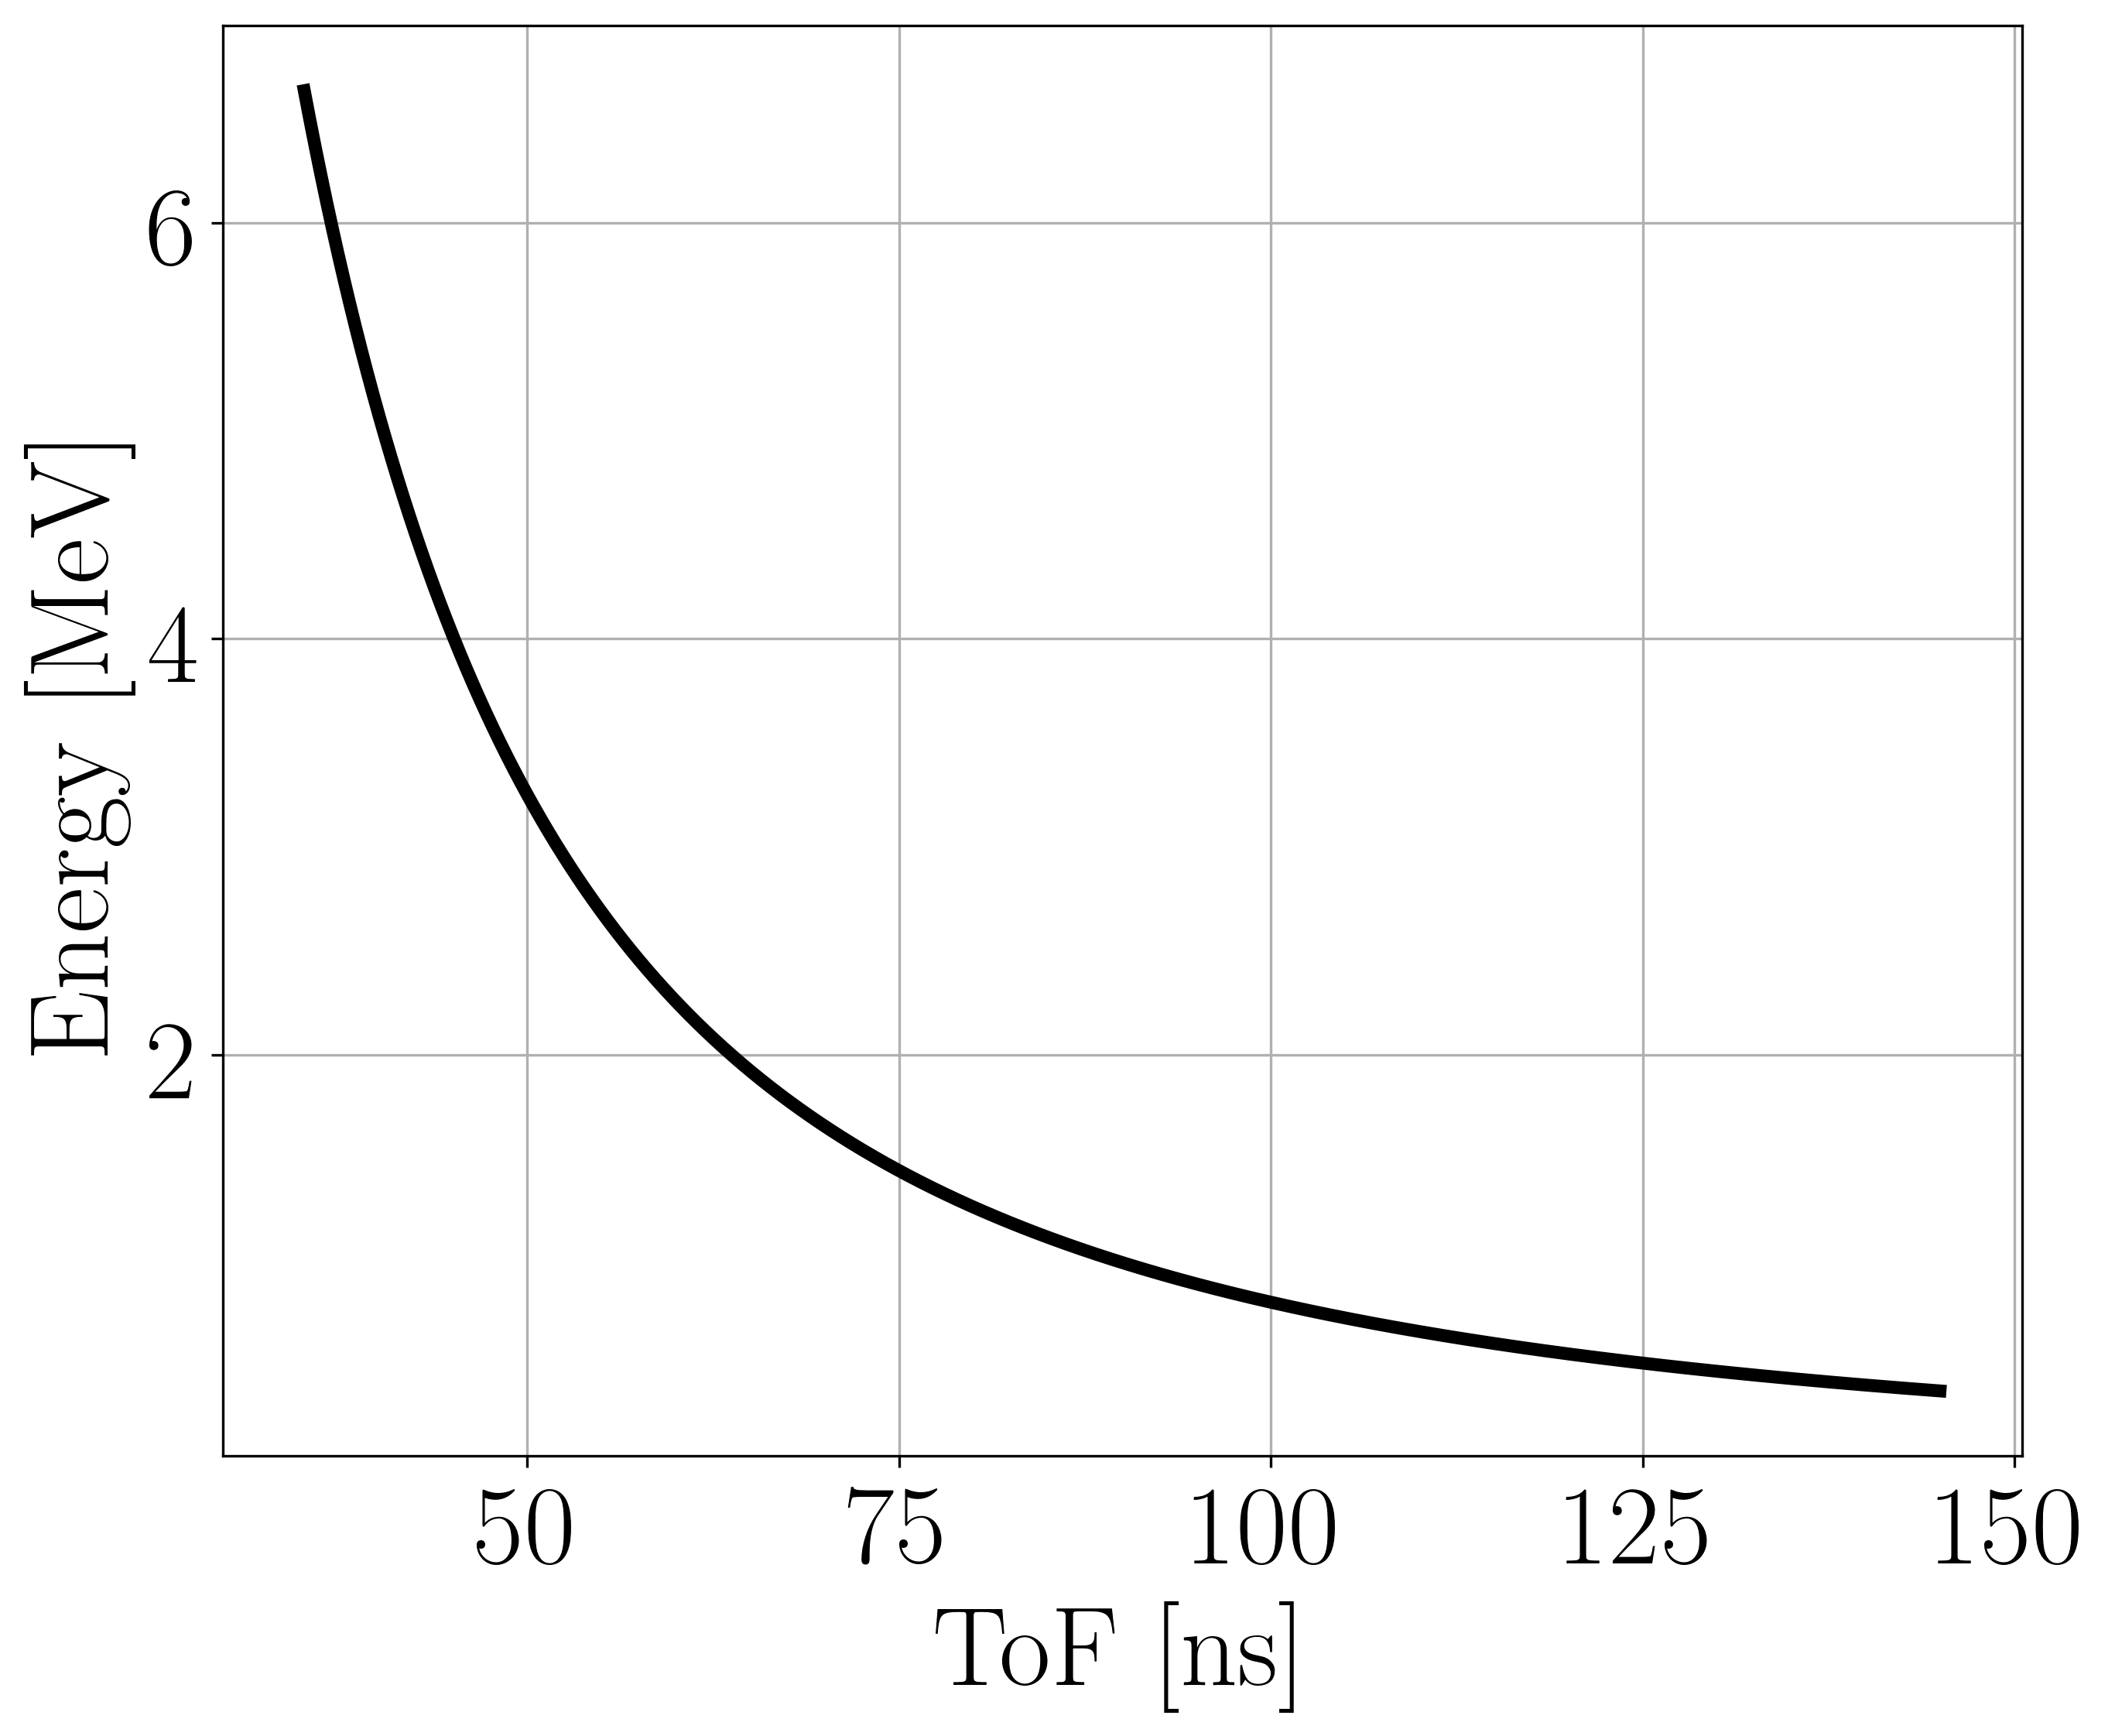
\includegraphics[width=\figsmall\textwidth]{ToF2Erg.png}}
    \subfloat[]{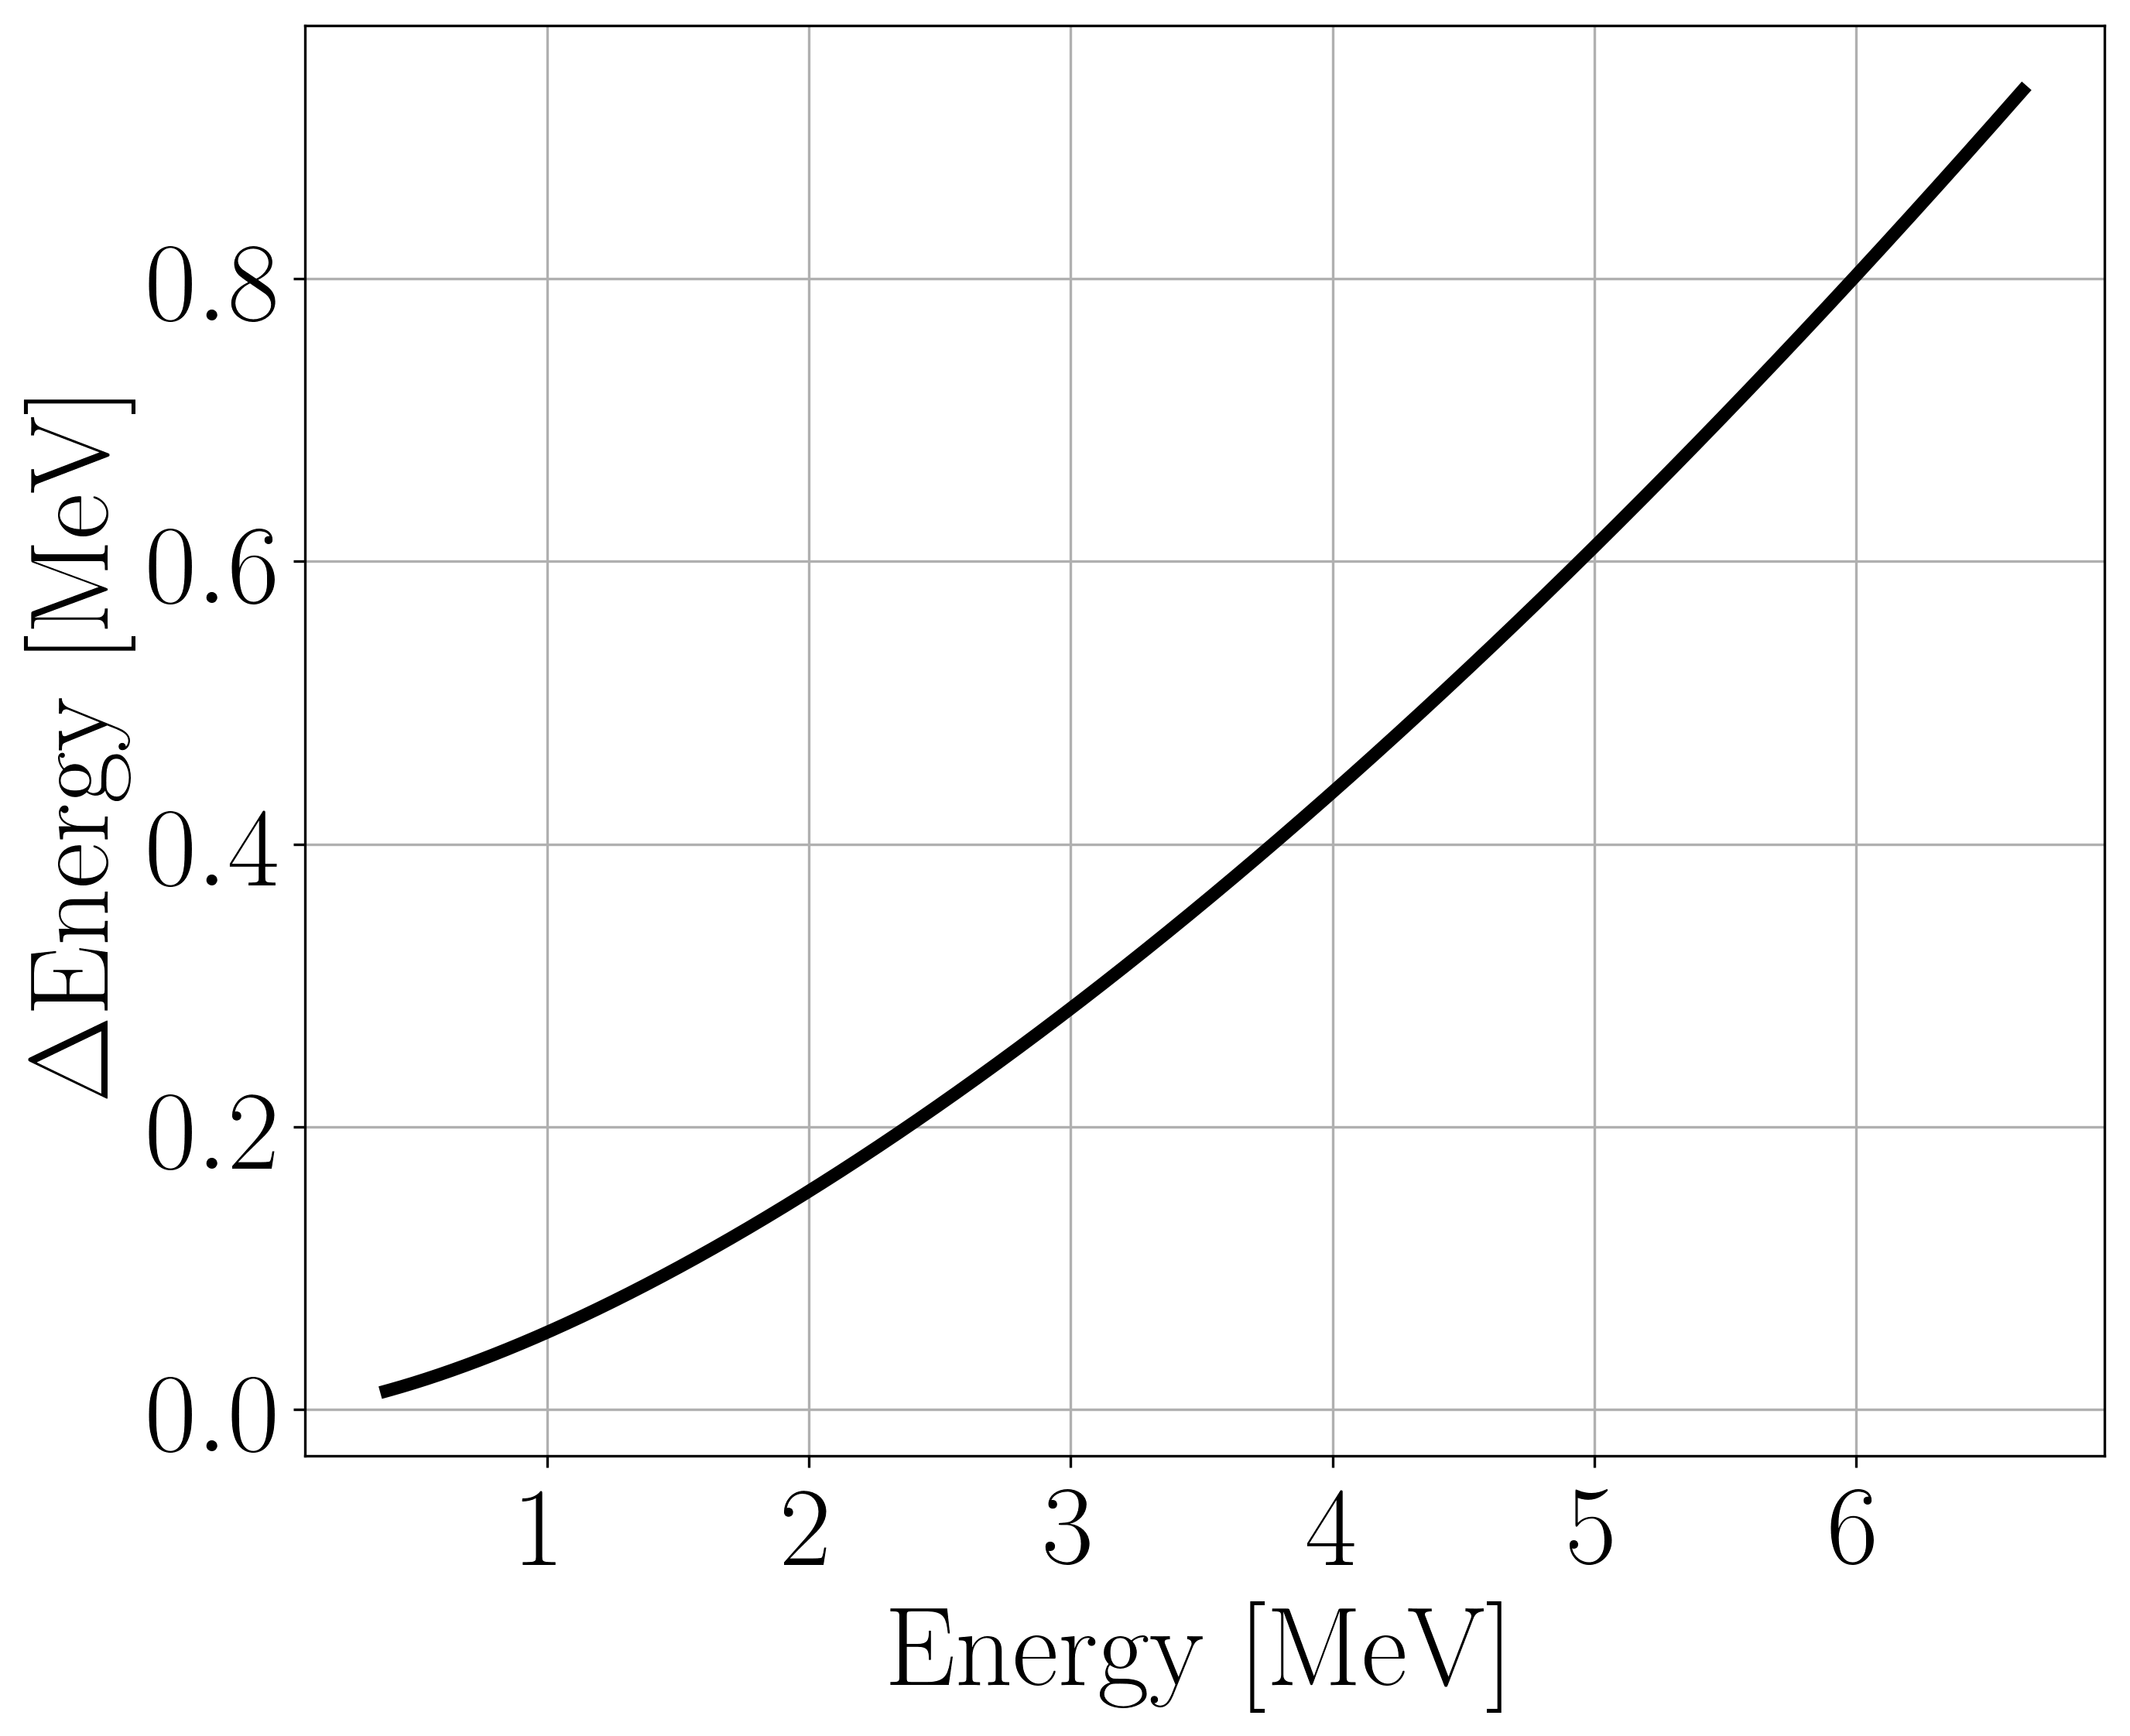
\includegraphics[width=\figsmall\textwidth]{DeltaErg.png}}
    \caption{%(a) Mapping from ToF to neutron energy: $E = \frac{8127}{ToF^{2}}$.
    Uncertainty in neutron energy measurements as a function of measured neutron energy.}
    \label{fig:ErgUncertainty}
\end{figure}
